\documentclass[11pt]{amsart}
\usepackage{geometry}                % See geometry.pdf to learn the layout options. There are lots.
\geometry{letterpaper}                   % ... or a4paper or a5paper or ... 
%\geometry{landscape}                % Activate for for rotated page geometry
%\usepackage[parfill]{parskip}    % Activate to begin paragraphs with an empty line rather than an indent
\usepackage{graphicx}
\usepackage{graphicx}
\usepackage{amssymb}
\usepackage{epstopdf}
\DeclareGraphicsRule{.tif}{png}{.png}{`convert #1 `dirname #1`/`basename #1 .tif`.png}

\title{Brief Article}
\author{The Author}
%\date{}                                           % Activate to display a given date or no date

\begin{document}
\maketitle
%\section{}
%\subsection{}

\section{Requirements for a programming language}

The programming model is based on cyclic graphs.
Graphs are kept distinct from each other. That is,
each graph is considered a self-contained
artifact, without links or pointers to other graphs.

A natural way to create such graphs is with 
imperative effects.

This potentially requires more copying of data
than would be the case in tree-based representations.

To modify graphs, place-holder objects are useful,
as is the ability to "become" another object.

\subsection{Simple reflection}

Fields can be created dynamically and accessed with
"." notation or reflective access.

\begin{verbatim}
o.foo   == o.get("foo")
\end{verbatim}

Assignment to fields can be overriden
\begin{verbatim}
   o.bar = 3   ==> o.set("bar", 3)
\end{verbatim}



\section{QuadModel}

\begin{figure}[htbp]
\begin{center}
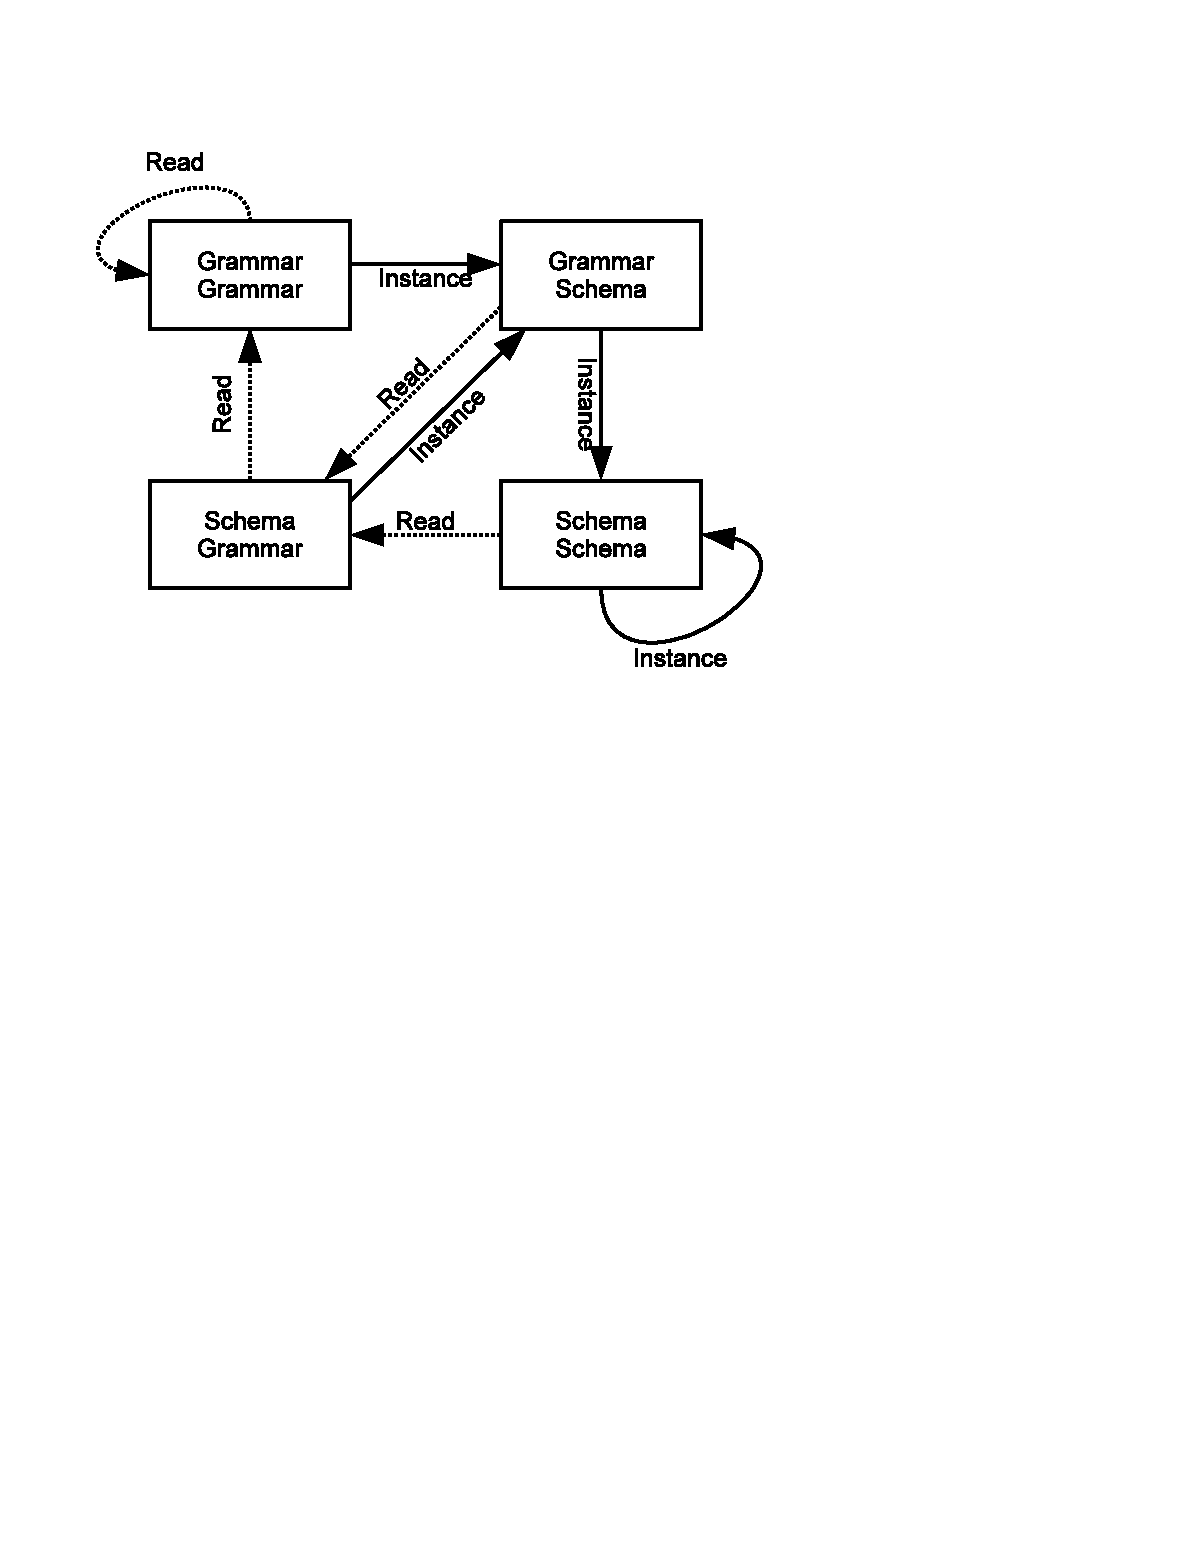
\includegraphics[scale=0.8]{QuadModel.eps}
\caption{{\bf default}}
\label{default}
\end{center}
\end{figure}



\end{document}  